\documentclass[12pt,a4paper]{article}

\usepackage{anysize}
\marginsize{3cm}{3cm}{3cm}{3cm}
\usepackage{graphicx}
\usepackage{t1enc}
\usepackage[MeX]{polski}
\usepackage[utf-8]{inputenc}
\usepackage[T1]{fontenc}
\usepackage{subfigure}

\usepackage{fancyhdr}
\setlength{\headheight}{15pt}
\pagestyle{fancy}

\newcommand{\HRule}{\rule{\linewidth}{0.5mm}}

\begin{document}

\begin{titlepage}

\begin{center}

% Upper part of the page

\includegraphics[width=0.15\textwidth]{./img/logo.eps}\\[1cm]

\textsc{\LARGE Akademia Górniczo-Hutnicza}\\[1.5cm]

\textsc{\Large Bazy Danych}\\[0.5cm]


% Title 
\HRule \\[0.4cm]
{ \huge \bfseries Rozkład Jazdy}\\[0.4cm]

\HRule \\[1.5cm]

% Author and supervisor
\begin{minipage}{0.4\textwidth}
\begin{flushleft} \large
\emph{Autorzy:}\\
Tomasz \textsc{Huczek}\\
Andrzej \textsc{Jasiński}
\end{flushleft}
\end{minipage}
\begin{minipage}{0.4\textwidth}
\begin{flushright} \large
\emph{Konsultant:} \\
prof. dr hab. inż. \\ Antoni \textsc{Ligęza}
\end{flushright}
\end{minipage}

\vfill

% Bottom of the page
{\large \today}

\end{center}

\end{titlepage}


\fancyhf{}

\lhead{Tomasz Huczek, Andrzej Jasiński}
\rhead{\today}
\rfoot{\thepage}

% \begin{abstract}
 Projekt konceptualny zawierający kolejne etapy projektowania i realizacji aplikacji bazy danych.
\end{abstract}


% \tableofcontents
% \newpage


\section{Sformułowanie zadania projektowego}
Podanie przedmiotu projektowania, jego celów,
przeglądu zadań, specyfiki i uwarunkowań.
\section{Analiza stanu wyjściowego}


%\textit{Analiza stanu zastanego, uwarunkowań prawnych, przyjętego
%obiegu istniejącej dokumentacji, analiza istniejącego systemu elektronicznego
%przetwarzania danych (aktualnej bazy), analiza występujących problemów, etc. pomocne
%mogą być scenariusze postępowania i ich analiza (elementy, obiekty, charakterystyki,
%atrybuty, struktura, przepływ danych, powiązania, relacje, ograniczenia funkcjonalności).} \\
Nasz system budujemy od podstaw, więc nie mamy żadnego istniejącego systemu badź dokumentacji. Oczywiście istnieją podobne rozwiązania,
jak np. strona krakowskiego MPK i chcemy osiągnąć podobną funkcjonalność. Niestety, z powodu pewnych ograniczeń samej bazy nie możemy na tym etapie wykonać pełnej implementacji wyszukiwarki połączeń.



\section{Analiza wymagań użytkownika}

\textit{Na tym etapie należy określić podstawowe
cele, zadania i funkcjonalność jakie mają być realizowane przez projektowaną bazę danych
oraz ew. wymagania dotyczące projektu i dokumentacji. Dobrze byłoby, aby użytkownik
na bieżąco współuczestniczył w projektowaniu i implementacji oraz wnosił swoje uwagi.
Należy zidentyfikować wymagania jawne i niejawne.} \\

Celem aplikacji oraz bazy danych jest zapewnienie jak największej wygody wyszukiwania informacji. Baza danych musi zapewnić możliwość wyszukiwania informacji w oparciu o kilka kryteriów. Użytkownik ma możliwość przeszukiwania lini autobusowych oraz przystanków. Linie autobusowe zawierają informacje przez jakie przystanki prowadzi dana linia oraz w jakich godzinach autobus przejeżdża przez dany przystanek. Informacje o przystankach to lista lini przejeżdżających przez dany przystanek oraz nazwa ulicy przy jakiej znajduje się przystanek.
\section{Określenie scenariuszy użycia}
Scenariusze użycia pozwolą na konstrukcję diagramów
DFD i STD oraz hierarchii funkcji.
\section{Identyfikacja funkcji}

% \textit{Określenie podstawowych funkcji realizowanych w bazie danych.} \\

Po wejściu na stronę WWW zwykły użytkownik ma jedynie możliwość przeglądania zawartości bazy, tj : poszukiwanie linii, rozkładów jazdy i przystanków. Administrator systemu może natomiast tworzyć nowe linie, przystanki, edytować już istniejące oraz usuwać. 
\section{Analiza hierarchii funkcji projektowanej aplikacji (FHD - Functional Hierarchy
Diagram)}
% \textit{Określenie struktury zależności hierarchicznych pomiędzy jednostkami
% analizowanego systemu, zwłaszcza w zakresie specyfikacji wymagań funkcjonalnych.
% Specyfikacja funkcji (funkcjonalności) projektowanego systemu.} \\
\renewcommand{\labelenumii}{\arabic{enumi}.\arabic{enumii}.}
\renewcommand{\labelenumiii}{\arabic{enumi}.\arabic{enumii}.\arabic{enumiii}.}

\begin{enumerate}
    \item Funkcje administratora
    \begin{enumerate}
        \item Zarządzanie liniami
                \begin{enumerate}
                    \item Dodawanie linii
                    \item Usuwanie linii
                    \item Edycja linii
                \end{enumerate}
        \item Zarządzanie przystankami
                \begin{enumerate}
                    \item Dodawanie nowego przystanku
                    \item Edycja istniejącego przystanku
                    \item Usuwanie przystanku
                \end{enumerate}
    \end{enumerate}

    \item Funkcje użytkownika
     \begin{enumerate}
        \item Przeszukiwanie bazy
            \begin{enumerate}
                \item Poszukiwanie możliwych połączeń pomiędzy dwoma przystankami
                \item Przeglądanie dostepnych linii
                \item Poszukiwanie przystanku według nazwy
                \item Poszukiwanie przystanku według nazwy ulicy
                \item Wyświetlenie rozkładu jazdy dla danej linii dla danego przystanku
            \end{enumerate}

     \end{enumerate}

\end{enumerate}





\section{Budowa i analiza diagramu przepływu danych - Data Flow Diagram }
\textit{Ma na celu określenie przepływu danych (wejścia, wyjścia, operacje, przechowywanie) oraz
elementów sterowania tym przepływem, co może być pomocne dla tworzenia aplikacji.
Specyfikacja danych wejściowych i wyjściowych.}

\section{Wybór encji (obiektów) i ich atrybutów}

\section{Projektowanie powiązań (relacji) pomiędzy encjami}

\textit{Konstrukcja diagramu ERD
(Entity-Relationship Diagram); jest to zasadniczy etap procesu projektowania struktury
bazy danych. Identyfikacja klas encji, ich atrybutów, zdefiniowanie (określenie) kluczy.
Tablica krzyżowa powiązań, eliminacja powiązań wiele-do-wielu. Konstrukcja diagramu
ERD.} \\


\section{Projekt diagramów STD (State Transition Diagram - diagramy przejść pomiędzy
stanami)}

\textit{Wykonanie w oparciu o scenariusze użycia i strukturę bazy danych. Pomocny do
budowy interfejsu aplikacji.} \\


\section{Projektowanie tabel, kluczy, kluczy obcych, powiązań między tabelami, indeksów, etc. w oparciu o zdefiniowany diagram ERD;} 

%na tym etapie następuje „sprecyzowanie” struktury bazy danych wraz ze szczegółami technicznymi. Projekt bazy w języku SQL.

%\begin{figure}[!htp]
%    \centering
%    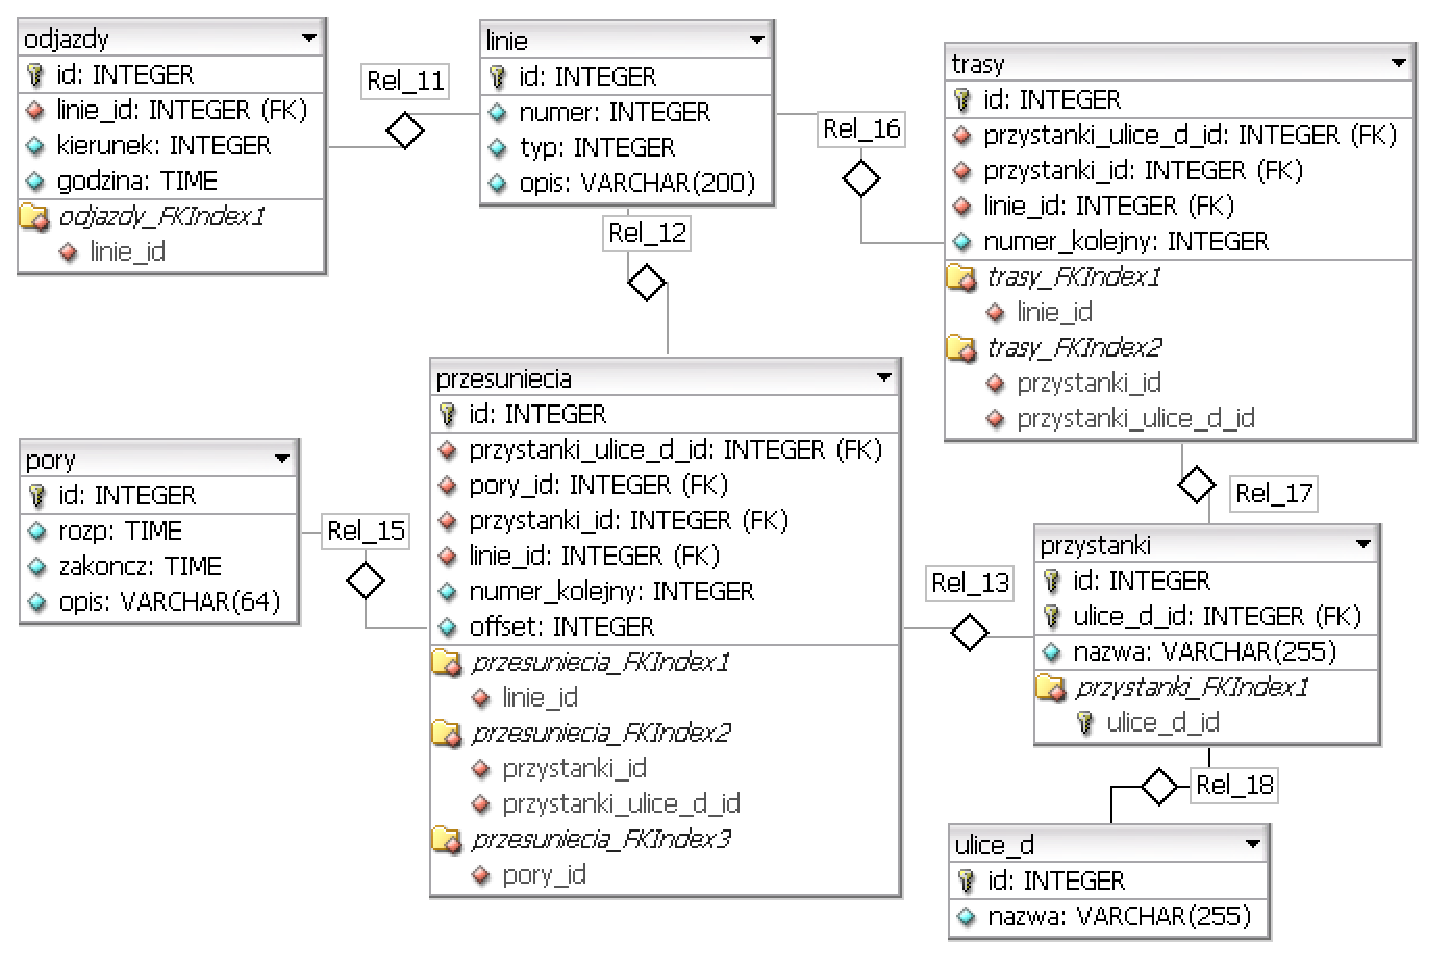
\includegraphics[width=0.75\textwidth]{./img/busag_model.eps}
%    \caption{Tabele}
%    \label{fig:tabs}
%\end{figure}

\begin{verbatim}
 CREATE TABLE linie (
    numer integer NOT NULL,
    typ integer NOT NULL,
    opis character varying(200)
);

CREATE TABLE odjazdy (
    id integer NOT NULL,
    linie_id integer NOT NULL,
    godzina time without time zone,
    kierunek bit(1) NOT NULL
);

CREATE TABLE pory (
    id integer NOT NULL,
    rozp time without time zone NOT NULL,
    zakoncz time without time zone NOT NULL,
    opis character varying(64) NOT NULL
);

CREATE TABLE przesuniecia (
    id integer NOT NULL,
    "offset" interval NOT NULL,
    trasy_id integer,
    powrotna bit(1) NOT NULL
);

CREATE TABLE przystanki (
    id integer NOT NULL,
    nazwa character varying NOT NULL,
    ulica1_id integer,
    ulica2_id integer
);

CREATE TABLE trasy (
    id integer NOT NULL,
    linie_id integer,
    przystanki_id integer,
    numer_kolejny integer
);

CREATE VIEW timetable_view AS
    SELECT odjazdy.linie_id AS linia_numer, trasy.numer_kolejny, przystanki.id AS przystanek_id, przystanki.nazwa AS przystanek, (przesuniecia."offset" + odjazdy.godzina) AS odj, odjazdy.id AS odj_id, odjazdy.kierunek FROM (((przesuniecia JOIN trasy ON ((przesuniecia.trasy_id = trasy.id))) JOIN przystanki ON ((trasy.przystanki_id = przystanki.id))) JOIN odjazdy ON ((odjazdy.linie_id = trasy.linie_id))) WHERE (odjazdy.kierunek = przesuniecia.powrotna) ORDER BY odjazdy.linie_id, trasy.numer_kolejny;


CREATE VIEW trasy_view AS
    SELECT trasy.przystanki_id, linie.numer, trasy.numer_kolejny, (SELECT przystanki.nazwa FROM przystanki WHERE (przystanki.id = trasy.przystanki_id)) AS nazwa FROM (trasy JOIN linie ON ((linie.numer = trasy.linie_id)));


ALTER TABLE ONLY linie
    ADD CONSTRAINT linie_numer_key UNIQUE (numer);

ALTER TABLE ONLY linie
    ADD CONSTRAINT linie_pkey PRIMARY KEY (numer);

ALTER TABLE ONLY odjazdy
    ADD CONSTRAINT odjazdy_pkey PRIMARY KEY (id);

ALTER TABLE ONLY pory
    ADD CONSTRAINT pory_pkey PRIMARY KEY (id);

ALTER TABLE ONLY przesuniecia
    ADD CONSTRAINT przesuniecia_pkey PRIMARY KEY (id);

ALTER TABLE ONLY przystanki
    ADD CONSTRAINT przystanki_nazwa_key UNIQUE (nazwa);

ALTER TABLE ONLY przystanki
    ADD CONSTRAINT przystanki_pkey PRIMARY KEY (id);

ALTER TABLE ONLY trasy
    ADD CONSTRAINT trasy_pkey PRIMARY KEY (id);

ALTER TABLE ONLY odjazdy
    ADD CONSTRAINT odjazdy_linie_id_fkey FOREIGN KEY (linie_id) REFERENCES linie(numer) ON UPDATE CASCADE ON DELETE CASCADE;

ALTER TABLE ONLY przesuniecia
    ADD CONSTRAINT przesuniecia_trasy_id_fkey FOREIGN KEY (trasy_id) REFERENCES trasy(id) ON UPDATE CASCADE ON DELETE CASCADE;

ALTER TABLE ONLY przystanki
    ADD CONSTRAINT przystanki_fk_id_ulica1_fkey FOREIGN KEY (ulica2_id) REFERENCES ulice_d(id);

ALTER TABLE ONLY przystanki
    ADD CONSTRAINT przystanki_fk_id_ulica2_fkey FOREIGN KEY (ulica1_id) REFERENCES ulice_d(id);

ALTER TABLE ONLY trasy
    ADD CONSTRAINT trasy_linie_id_fkey FOREIGN KEY (linie_id) REFERENCES linie(numer) ON UPDATE CASCADE ON DELETE CASCADE;

ALTER TABLE ONLY trasy
    ADD CONSTRAINT trasy_przystanki_id_fkey FOREIGN KEY (przystanki_id) REFERENCES przystanki(id) ON UPDATE CASCADE ON DELETE RESTRICT;
\end{verbatim}




\section{Słowniki danych.}
W naszym projekcie znajdują się dwa słowniki danych:
\begin{itemize}
 \item Słownik nazw ulic, który będzie używany podczas wyszukiwania i pokazywania ulic (a dokładniej skrzyżowań) podczas przeglądania bądź szukania przystanku.
\end{itemize}

Słownik jest zdefiniowane w postaci tabeli zawierającej klucz główny (ID) oraz kolumnę typu VARCHAR z nazwą.
\section{Projektowanie operacji na danych: zdefiniowanie kwerend dla realizacji funkcji wyspecyfikowanych w projekcie}




\clearpage
% \addcontentsline{toc}{section}{Literatura}
% \begin{thebibliography}{99}
% \bibitem{bib:onelecture} Jakaś książka
% \end{thebibliography}

\end{document}
